There were 98 registered participants with skill demographics illustrated in Fig. \ref{Fig:skilldemo}. When inviting participants to the hackathon, a diverse skill set was encouraged for inter-disciplinary project collaboration on security solutions. This includes the following: Security-oriented participants (non-technical cybersecurity or data protection professionals, cybersecurity experts, and students willing to learn about cybersecurity), software development oriented participants (Data specialist, UI/UX designers, front-end developers, back-end developers), and product oriented participants (visionaries, marketing gurus and passionate project managers). Bringing together these set of diverse participants allow implementation of ideas from various perspectives, and facilitate spontaneous collaborative learning among the participants\cite{pe2018designing}.




\begin{figure}[h]
%\vspace{-15pt}
  \centering
  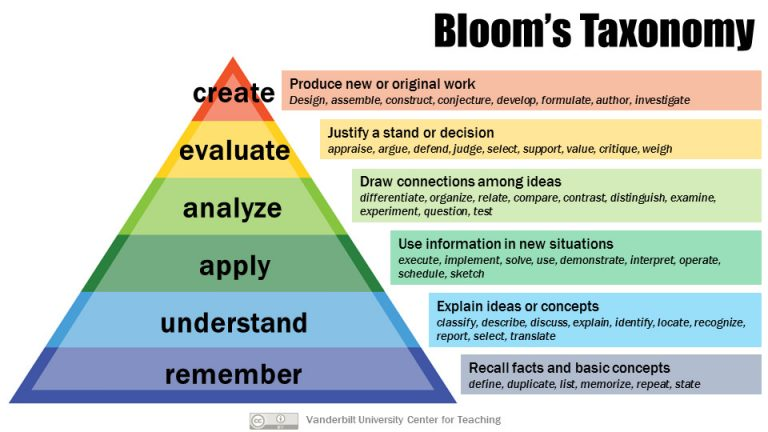
\includegraphics[width=\linewidth]{Blooms-Taxonomy.jpg}
  \caption{Hackathons in Security} \label{Fig:hackcycle} 
 % \vspace{-20pt}
\end{figure}

The revised Blooms taxonomy %consists of six major categories that describe the cognitive processes by which a person involved in a learning environment encounter and work with knowledge.
is based on the two parts of educational objectives: (1) the \textbf{knowledge dimension} - nouns describing the content (knowledge) to be learned, and (2) the \textbf{process dimension} - verbs describing the processes students use in producing or working with knowledge.


\subsubsection{The knowledge dimension}
This includes the content aspect of the remembering process of the blooms taxonomy, separated into factual, conceptual, procedural and meta-cognitive knowledge categories.

\begin{itemize}
    \item Factual Knowledge: This includes the the basic elements students must know to be acquainted with a discipline or solve problems in it, e.g, knowledge of terminology or specific details. This influences the students ability to list, summarize, classify, order, rank or contribute to the basic elements within a specific discipline.
    \item Conceptual Knowledge: This is knowledge of the interrelationships among the basic elements within a larger structure that enable them to function together, e.g, knowledge of classification and categories, principles and generalizations, and theories, models and structures. It influences the students ability to describe, interpret, experiment, explain assess or plan
    \item Procedural Knowledge: This is knowledge gained through thinking, experience, and the use of the senses, e.g, strategic knowledge, self-knowledge.
\end{itemize}

\subsubsection{The process dimension}

\begin{itemize}
    \item Remembering: Retrieving, recognizing, and recalling relevant knowledge from long-term memory.
    \item Understanding: Constructing meaning from oral, written, and graphic messages through interpreting, exemplifying, classifying, summarizing, inferring, comparing, and explaining.
    \item Applying: Carrying out or using a procedure through executing, or implementing.
    \item Analyzing: Breaking material into constituent parts, determining how the parts relate to one another and to an overall structure or purpose through differentiating, organizing, and attributing.
    \item Evaluating: Making judgments based on criteria and standards through checking and critiquing.
    \item Creating: Putting elements together to form a coherent or functional whole; reorganizing elements into a new pattern or structure through generating, planning, or producing.
\end{itemize}

\begin{table*}[h]
    \centering
    \begin{tabular}{|p{0.2\linewidth}|p{0.12\linewidth}|p{0.1\linewidth}|p{0.1\linewidth}|p{0.1\linewidth}|p{0.1\linewidth}|p{0.1\linewidth}|}
    \hline
      & \multicolumn{6}{c|}{\textbf{The cognitive process dimension}}  \\ \hline
	\textbf{The knowledge dimension} & Remember & Understand  & Apply & Analyse & Evaluate & Create \\ \hline
	Factual Knowledge & List & Summarize & Classify & Order & Rank & Combine \\ \hline
	Conceptual & Describe & Interpret & Experiment & Explain & Assess & Plan \\ \hline
	Procedural & Tabulate & Predict & Calculate & Differentiate & Conclude & Compose \\ \hline
	Meta-cognitive & Appropriate use & Execute & Construct & Achieve & Action & Actualise \\ \hline
    \end{tabular}
    \caption{Blooms Taxonomy categories}
    \label{tab:bloomsubcategories}
\end{table*}
